% This work is licensed under the Creative Commons
% Attribution-NonCommercial 3.0 Unported License. To view a copy of this
% license, visit http://creativecommons.org/licenses/by-nc/3.0/.

\section{Auswertung}
%
\subsection{Untersuchung eines Reflexklystrons}
%
\subsubsection{Untersuchung der Moden auf einem Oszilloskop}
%
Das Vermessen dreier verschiedener Moden des Klystrons liefert 
die in Tabelle~\ref{tab:moden} eingetragenen Werte für die 
Mittenfrequenzen $f_0$, den Amplituden $A_0$ und den 
Reflektorspannungen $V_0$, $V_1$ und $V_2$ der untersuchten 
Moden. Die Reflektorspannungen werden pro Mode so eingestellt, 
dass sich diese auf dem Oszilloskop, wie im Durchführungsabschnitt 
4.1 erklärt, zeigen.

Die Frequenzen sind nicht fehlerbehaftet, da es möglich ist, mit dem 
Frequenzmesser die Anzeige auf \SI{1}{\mega\hertz} genau 
einzustellen. Wie im Diskussionsteil zu den Frequenzmessungen 
erwähnt, muss dies aber nicht die tatsächliche Frequenz der 
Mikrowelle sein!

\begin{table}[h]
  \centering
  \sisetup {
    per-mode = fraction
  }
  \begin{tabular}{SSSSSS}
    \toprule
    {Mode}&
    {$V_0$}{/}\si{\volt}&{$V_1$}{/}\si{\volt}&{$V_2$}{/}\si{\volt}& 
    {$A_0$}{/Teilstriche}&{$f_0$}{/}\si{\mega\hertz}\\
    \midrule
    1&215(5)&200(5)&230(5)&3.2(1)&9000\\
    2&140(5)&120(5)&150(5)&3.1(1)&9005\\
    3&85(5)&70(5)&100(5)&2.4(1)&9010\\
    \bottomrule
  \end{tabular}
  \caption{Mithilfe eines Oszilloskops abgelesene 
               Werte für verschiedene Moden des Klystrons. 
Die verschiedenen Moden werden ebenfalls mithilfe des Oszilloskops 
eingestellt. Die Fehler ergeben sich aus der Ablesegenauigkeit von den 
Messgeräten.}
  \label{tab:moden}
\end{table}

Es werden pro Mode drei Reflektorspannungen gemessen, 
um daraus das Diagramm in Abb.\ref{fig:moden} erstellen zu können.
In diesem Diagramm ist der Zusammenhang zwischen der 
eingestellten Reflektorspannung und der Leistung der verschiedenen 
Moden zu sehen.

\begin{figure}[]
  \centering
  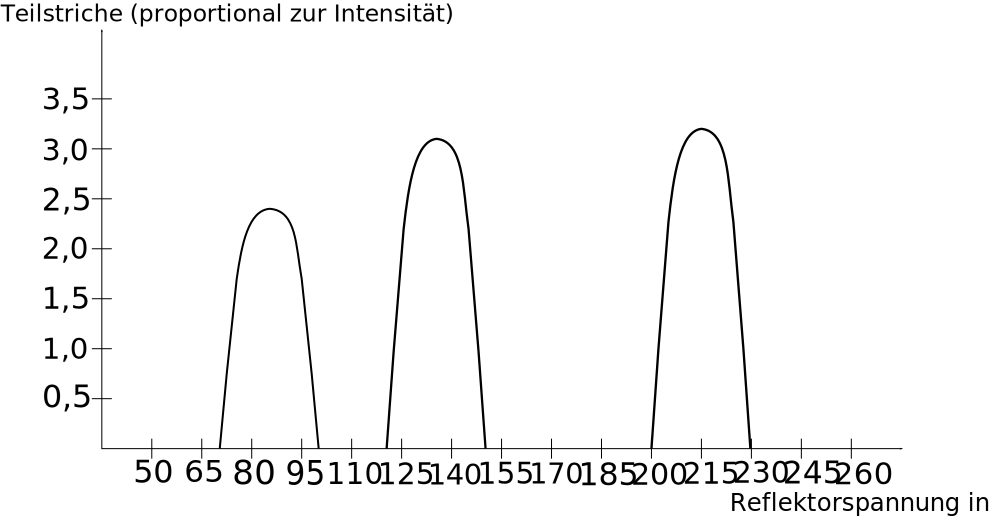
\includegraphics[width=0.9\textwidth]{modenbild.pdf}
  \caption{Plot der Intensität verschiedener Mikrowellenmoden 
               des Klystrons gegen die angelegte Reflektorspannung.
               Da die Intensität proportional zu der auf dem 
               Oszilloskop angezeigten Amplitude ist, dienen 
                die Teilstriche als Maß der Intensität.}
  \label{fig:moden}
\end{figure}
\FloatBarrier
%
\subsubsection{Elektronische Abstimmung}
%
Die höchste Mode mit einer Frequenz von \SI{9001}{\mega\hertz} 
liefert bei Verschiebung der Anzeige des Oszilloskops durch Variation 
der Reflektorspannung die in Tabelle~\ref{tab:abstimm} gezeigten 
Werte. Die Modenanzeige wird dabei ebenfalls so verschoben, wie 
es im Durchführungsteil 4.1 erläutert wird.

\begin{table}[h]
  \centering
  \sisetup {
    per-mode = fraction
  }
  \begin{tabular}{cSS}
    \toprule
    Modeneinstellung&
    {Reflektorspannung}{/}\si{\volt}&
   {Frequenz}{/}\si{\mega\hertz}\\
    \midrule
    a&215(5)&9001\\
    b&200(5)&8982\\
    c&225(5)&9022\\
    \bottomrule
  \end{tabular}
  \caption{Zur Ermittlung der Abstimm-Empfindlichkeit 
               aufgenommene Messwerte.}
  \label{tab:abstimm}
\end{table}

Aus den Werten in Tabelle~\ref{tab:abstimm} wird die 
Abstimm-Empfindlichkeit mittels Formel~\eqref{eq:abstimm} 
bestimmt. Der dort angegebene Fehler stammt aus einer 
Gausschen Fehlerfortpflanzung, wobei $V_c$ und $V_b$ die 
mit den in Tabelle~\ref{tab:abstimm} angegebenen Fehlern 
fehlerbehafteten Werte sind.

\begin{equation}
\text{Abstimm-Empfindlichkeit }A=\frac{f_c - f_b}{V_c - V_b} =
\SI{1.6(5)}
{\mega\hertz\per\volt}
\label{eq:abstimm}
\end{equation}
%
Die elektronische Bandbreite liest man hieraus zu 
\begin{equation*}
f_c - f_b = \SI{40}{\mega\hertz}
\end{equation*}
ab.
\FloatBarrier
%
\subsection{Messung von Frequenz, Wellenlänge und Dämpfung}
%
\subsubsection{Frequenzmessung}
%
Die direkte Frequenzmessung mit dem Frequenzmesser ergibt 
die Frequenz $f_\text{direkt}$ in Tabelle~\ref{tab:freq}. 

Die benötigte Wellenlänge der stehenden Welle $\lambda_g$ und die 
Innenabmessung des Hohlleiters a für eine rechnerische Bestimmung 
der Frequenz $f_\text{rechnung}$ der 
eingestellten Mikrowelle sind ebenfalls in Tabelle~\ref{tab:freq} zu 
sehen. Auch die daraus berechnete Frequenz
\begin{equation}
f = c\cdot\sqrt{\left(\frac{1}{\lambda_g}\right)^2 + \left(\frac{1}{2a}\right)^2}
\label{eq:label}
\end{equation} 
ist in dieser Tabelle eingetragen.

\begin{table}[h]
  \centering
  \sisetup {
    per-mode = fraction
  }
  \begin{tabular}{SSSS}
    \toprule
    {$f_\text{direkt}$/}\si{\mega\hertz}&
    {$\lambda_g$}{/}\si{\milli\metre}&
   {a}{/}\si{\milli\metre}&
    {$f_\text{rechnung}$/}\si{\mega\hertz}\\
    \midrule
    8994&48,0(1)&22.5(1)&9132(44)\\
    \bottomrule
  \end{tabular}
  \caption{Direkte und über stehende Wellen bestimmte Frequenzen 
               der sich im Hohlleiter befindlichen Mikrowelle. Die 
               erhaltenen Werte weichen stark voneinander ab.
               Wellenlängen- und Abmessungsfehler sind durch die an 
                den Messgeräten angebrachten Nonien gegeben. Der 
                 Fehler von $f_\text{rechnung}$ ergibt sich dann aus 
einer Fehlerfortpflanzung von~\eqref{eq:label}.}
  \label{tab:freq}
\end{table}
\FloatBarrier
%
\subsubsection{Dämpfungsmessung}
%
Über die Methode der Leistungsverhältnisse werden die Werte 
der Dämpfung gemessen, welche in Tabelle~\ref{tab:daempfung} 
eingetragen sind.
Ebenso in dieser Tabelle sind die Werte der auf dem einstellbaren 
Dämpfungsglied angebrachten Eichkurve.

Da der \SI{0}{\decibel}-Messausschlag auf dem SWR-Meter 
so liegt, dass das Dämpfungsglied eine Dämpfung von 
\SI{9}{\decibel} anzeigt, muss auf die gemessene Dämpfung 
\SI{9}{\decibel} addiert werden, um gemessene Dämpfung 
und Eichkurve auf dem Dämpfungsglied vergleichen zu können. 
Dies wird in Abbildung~\ref{fig:daempfung} beachtet.

\begin{table}[h]
  \centering
  \sisetup {
    per-mode = fraction
  }
  \begin{tabular}{SSSS}
    \toprule
    {SWR-Anzeige/}\si{\decibel}&
    {Mikrometerposition/}\si{\milli\metre}&
   {Eichkurvendämpfung/}\si{\decibel}\\
    \midrule
    0&2.14(2)&9.0(5)\\
    2&2.54(2)&11.5(5)\\
    4&2.86(2)&15.0(5)\\
    6&3.26(2)&20.0(5)\\
    8&3.58(2)&23.5(5)\\
    10&3.96(2)&29.0(5)\\
    \bottomrule
  \end{tabular}
  \caption{Die Untersuchung der Dämpfung des Dämpfungsgliedes 
               mit einem SWR-Meter über die Methode der 
               Leistungsverhältnisse liefert die Dämpfungswerte der 
               linken Spalte. Die Eichkurve, welche auf dem 
               Dämpfungsglied angebracht ist, gibt hingegen die 
               Dämpfung der rechten Spalte an.}
  \label{tab:daempfung}
\end{table}

\begin{figure}[]
  \centering
  \includegraphics[width=0.8\textwidth]{daempfung.pdf}
  \caption{Vergleich zwischen mit dem SWR-Meter gemessener 
               Dämpfung des Dämpfungsgliedes und den auf der  
               Eichkurve abgelesenen Dämpfungswerten für 
               verschiedene Mikrometerschraubenstellungen.}
  \label{fig:daempfung}
\end{figure}
\FloatBarrier
%
\subsection{Stehwellenmessungen}
%
\subsubsection{Messung von kleinen und mittleren Welligkeiten}
%
Das mit dem SWR-Meter bestimmte SWR für verschiedene Sondentiefen 
des Gleitschraubentransformators ist in Tabelle~\ref{tab:welligkeitklein} 
zu sehen.

\begin{table}[h]
  \centering
  \sisetup {
    per-mode = fraction
  }
  \begin{tabular}{SSSS}
    \toprule
    {Sondentiefe/}\si{\milli\metre}&
    {SWR}\\
    \midrule
    3&1.1\\
    5&1.5\\
    7&3.5\\
    9&$\infty$\\
    \bottomrule
  \end{tabular}
  \caption{Direkte SWR-Messung mittels SWR-Meter für 
               verschiedene Sondentiefen des 
               Gleitschraubentransformators. Größere Sondentiefen 
               führen zu größeren Welligkeiten.}
  \label{tab:welligkeitklein}
\end{table}
\FloatBarrier
%
\subsubsection{Messen großer Welligkeiten}
%
Um das SWR für eine Sondentiefe von \SI{9}{\milli\metre} 
zu bestimmen, wird zum einen die \SI{3}{\decibel}-Methode und 
zum anderen die Abschwächer-Methode verwendet.

In Tabelle~\ref{tab:welligkeitgross} sind alle benötigten Größen 
beider Methoden eingetragen, sowie das sich jeweils ergebende SWR. 
Für die \SI{3}{\decibel}-Methode sind die beiden Positionen der 
Meßleitungssonde $d_1$ und $d_2$, sowie die Wellenlänge der 
Mikrowelle $\lambda_g$ eingetragen, welche mit Hilfe von 
Formel~\eqref{eq:dreidb} das SWR ergeben.
Die Abschwächer-Methode ergibt mit den Dämpfungen $A_1$ und $A_2$ 
und Formel~\eqref{eq:abschwächer} das SWR, wobei die Dämpfungen 
so zu bestimmen sind, wie es im dazugehörigen Durchführungsteil 
erläutert wird.

\begin{table}[h]
  \centering
  \sisetup {
    per-mode = fraction
  }
  \begin{tabular}{SSSS}
    \toprule
    \multicolumn{4}{c}{\SI{3}{\decibel}-Methode}\\
    {$d_1$/}\si{\milli\metre}&{$d_2$/}\si{\milli\metre}&
    {$\lambda_g$/}\si{\milli\metre}&{SWR}\\
    \midrule
    100,0(1)&98,0(1)&48,0(1)&437.7(1)\\
    \midrule
    \multicolumn{4}{c}{Abschwächer-Methode}\\
    {$A_1$/}\si{\decibel}&{$A_2$/}\si{\decibel}&
    {$A_1-A_2$/}\si{\decibel}&{SWR}\\
    \midrule
    20,0(5)&38,0(5)&18,0(5)&9,0(4)\\
    \bottomrule
  \end{tabular}
  \caption{Die bei einer Sondentiefe von \SI{9}{\milli\metre} 
               ermittelten Welligkeiten mittels zweier Methoden. 
               Bei der \SI{3}{\decibel}-Methode wird 
               Formel~\eqref{eq:dreidb} verwendet, um das SWR 
               zu errechnen, bei der Abschwächer-Methode 
               Formel~\eqref{eq:abschwächer}. Die Fehler der SWR 
               ergeben sich dann aus den jeweiligen 
               Fehlerfortpflanzungen.}
  \label{tab:welligkeitgross}
\end{table}

\begin{equation}
\text{SWR}_{\SI{3}{\decibel}} = \sqrt{1+ \frac{1}{\sin^2
{\left(\frac{\pi(d_1-d_2)}{\lambda_g}\right)}}}
\label{eq:dreidb}
\end{equation}

\begin{equation}
\text{SWR}_\text{abschwächer} = 10\cdot\frac{A_2-A_1}{20}
\label{eq:abschwächer}
\end{equation}
\FloatBarrier
%